\documentclass[varwidth, border=0pt]{standalone}

\usepackage{times}      % Loads the Times-Roman Fonts
\usepackage{mathptmx}   % Loads the Times-Roman Math Fonts
\usepackage{subcaption}
\usepackage[labelfont={bf,sf},%
labelsep=period,%
justification=centering,
labelformat=parens,labelsep=quad,skip=3pt,font=scriptsize]{caption}
\usepackage{graphicx}

\begin{document}
	
	\begin{figure}
	\centering
\begin{subfigure}{\linewidth}
	\centering
	\vspace*{-6pt}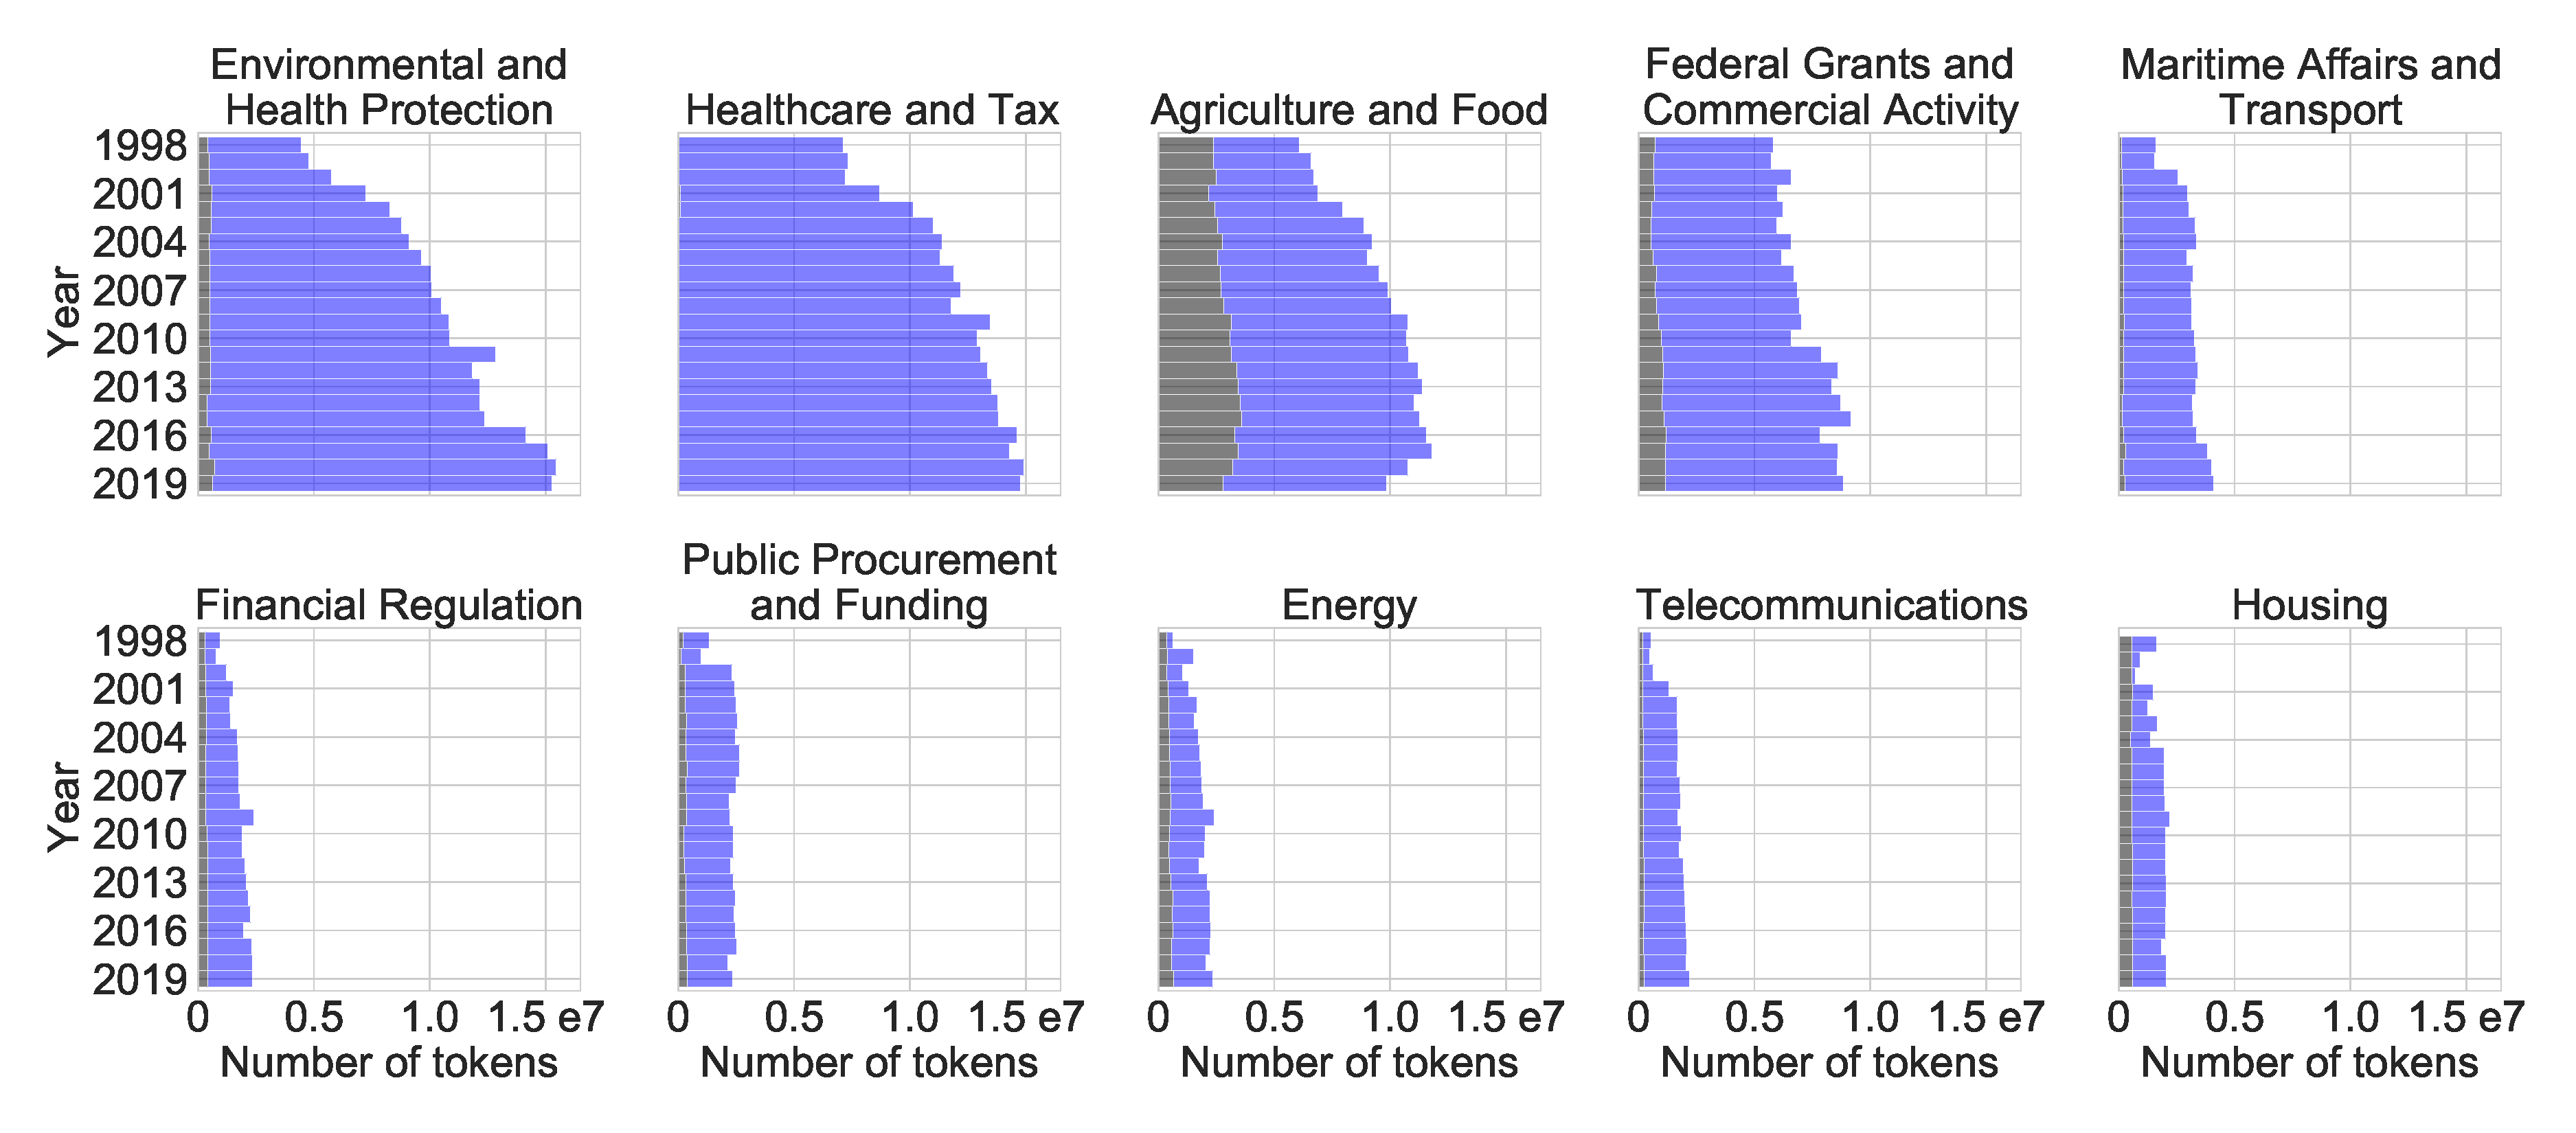
\includegraphics[width=\linewidth]{../../graphics/family-composition-absolute-n100-us.pdf}\vspace{-7pt}
	\vspace*{-6pt}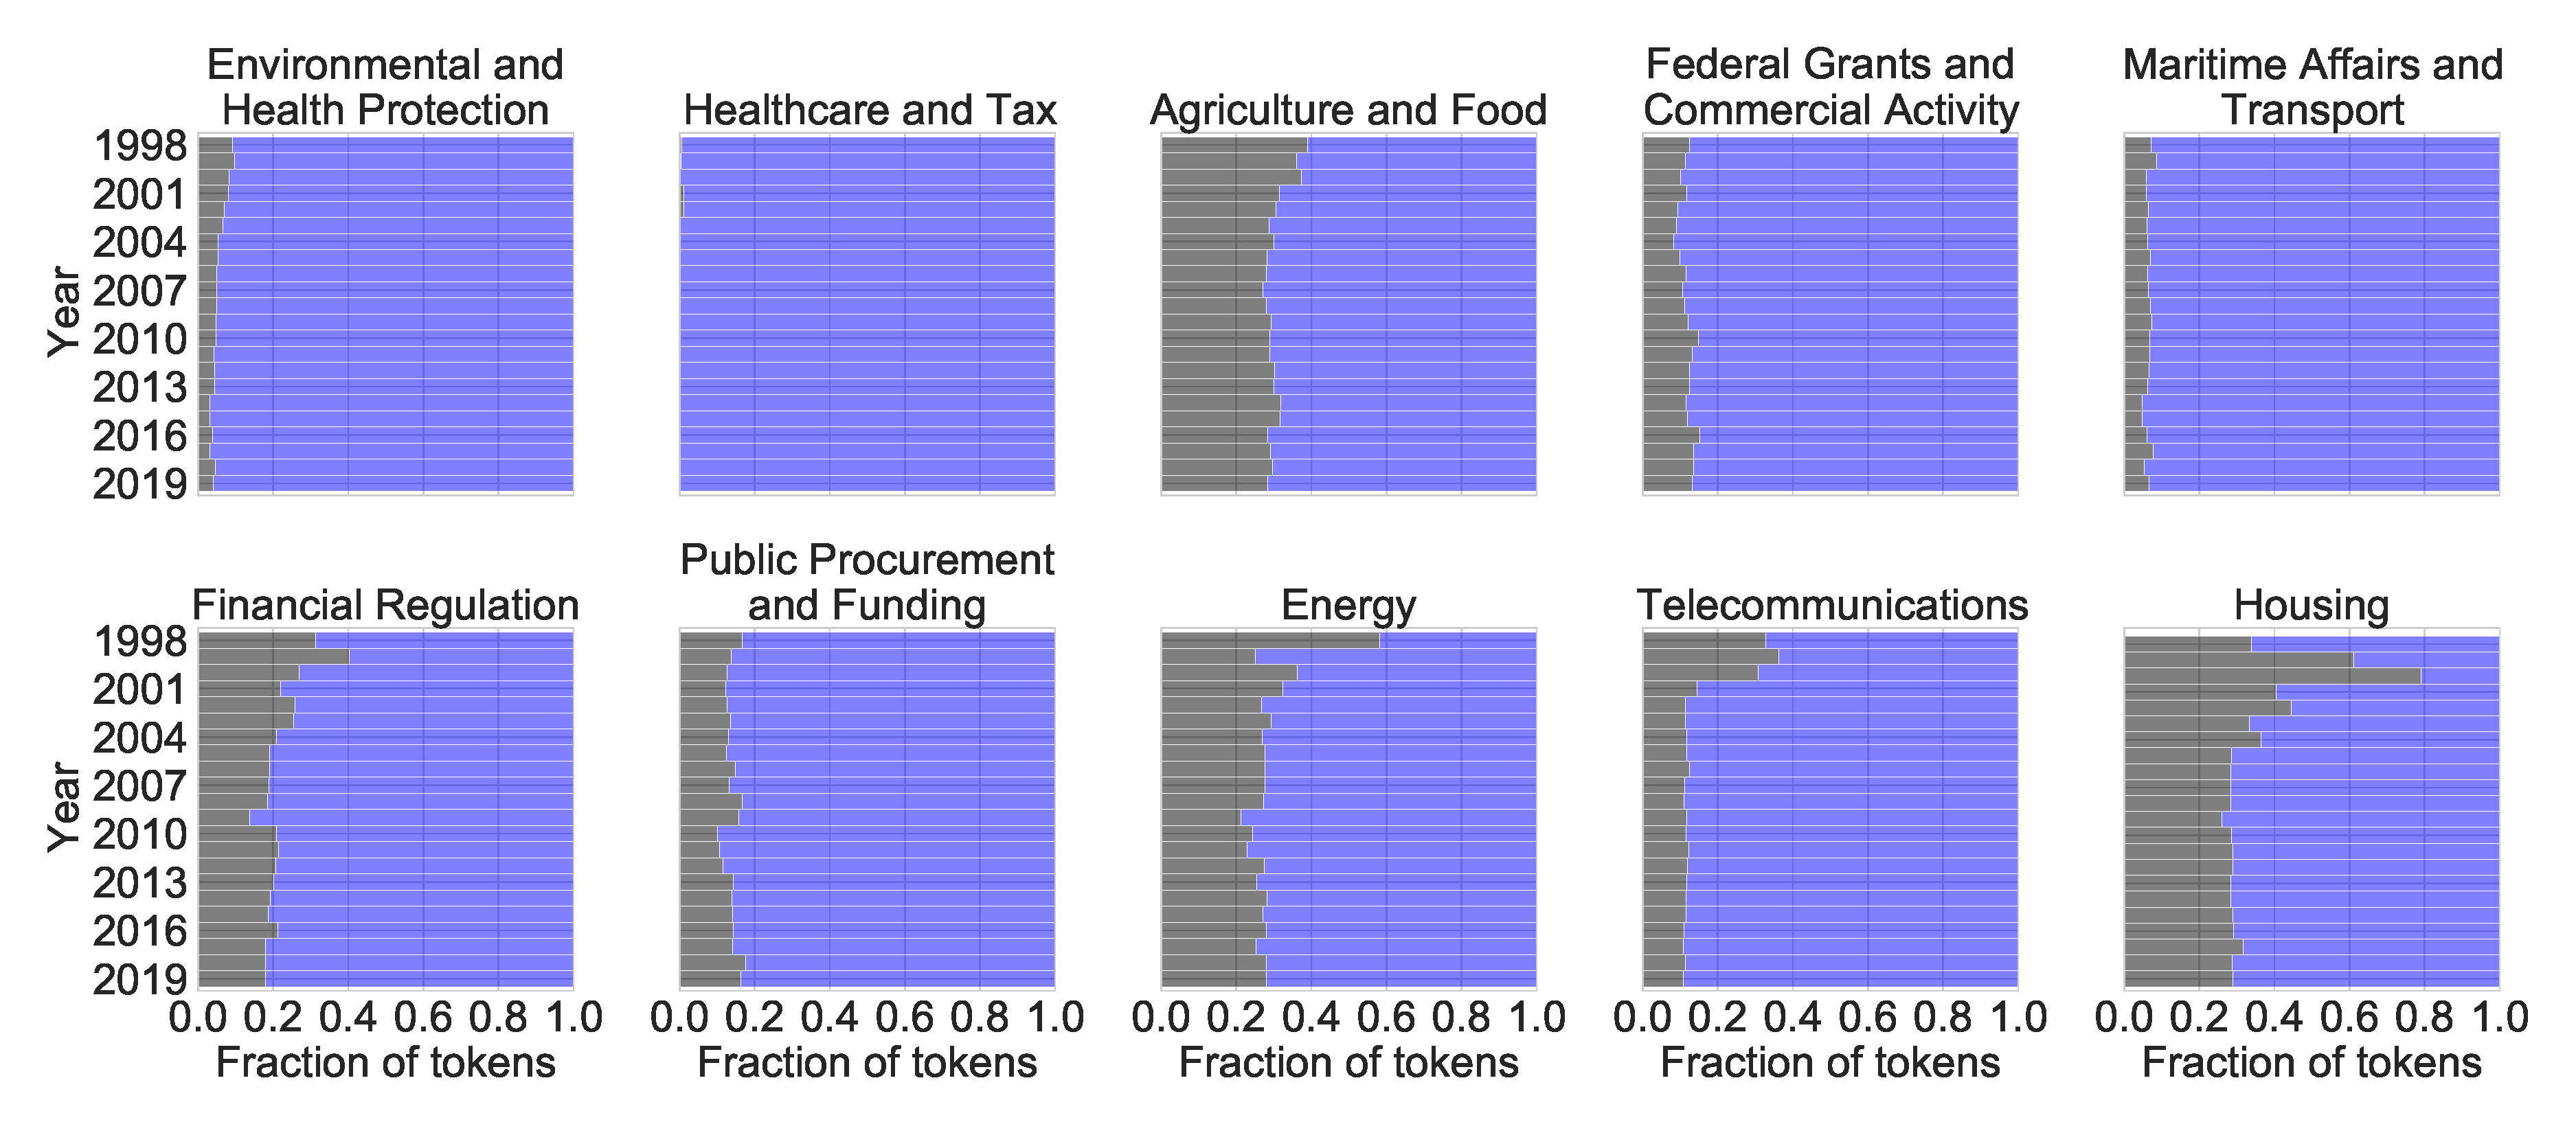
\includegraphics[width=\linewidth]{../../graphics/family-composition-relative-n100-us.pdf}
	\subcaption{United States}
\end{subfigure}

\begin{subfigure}{\linewidth}
	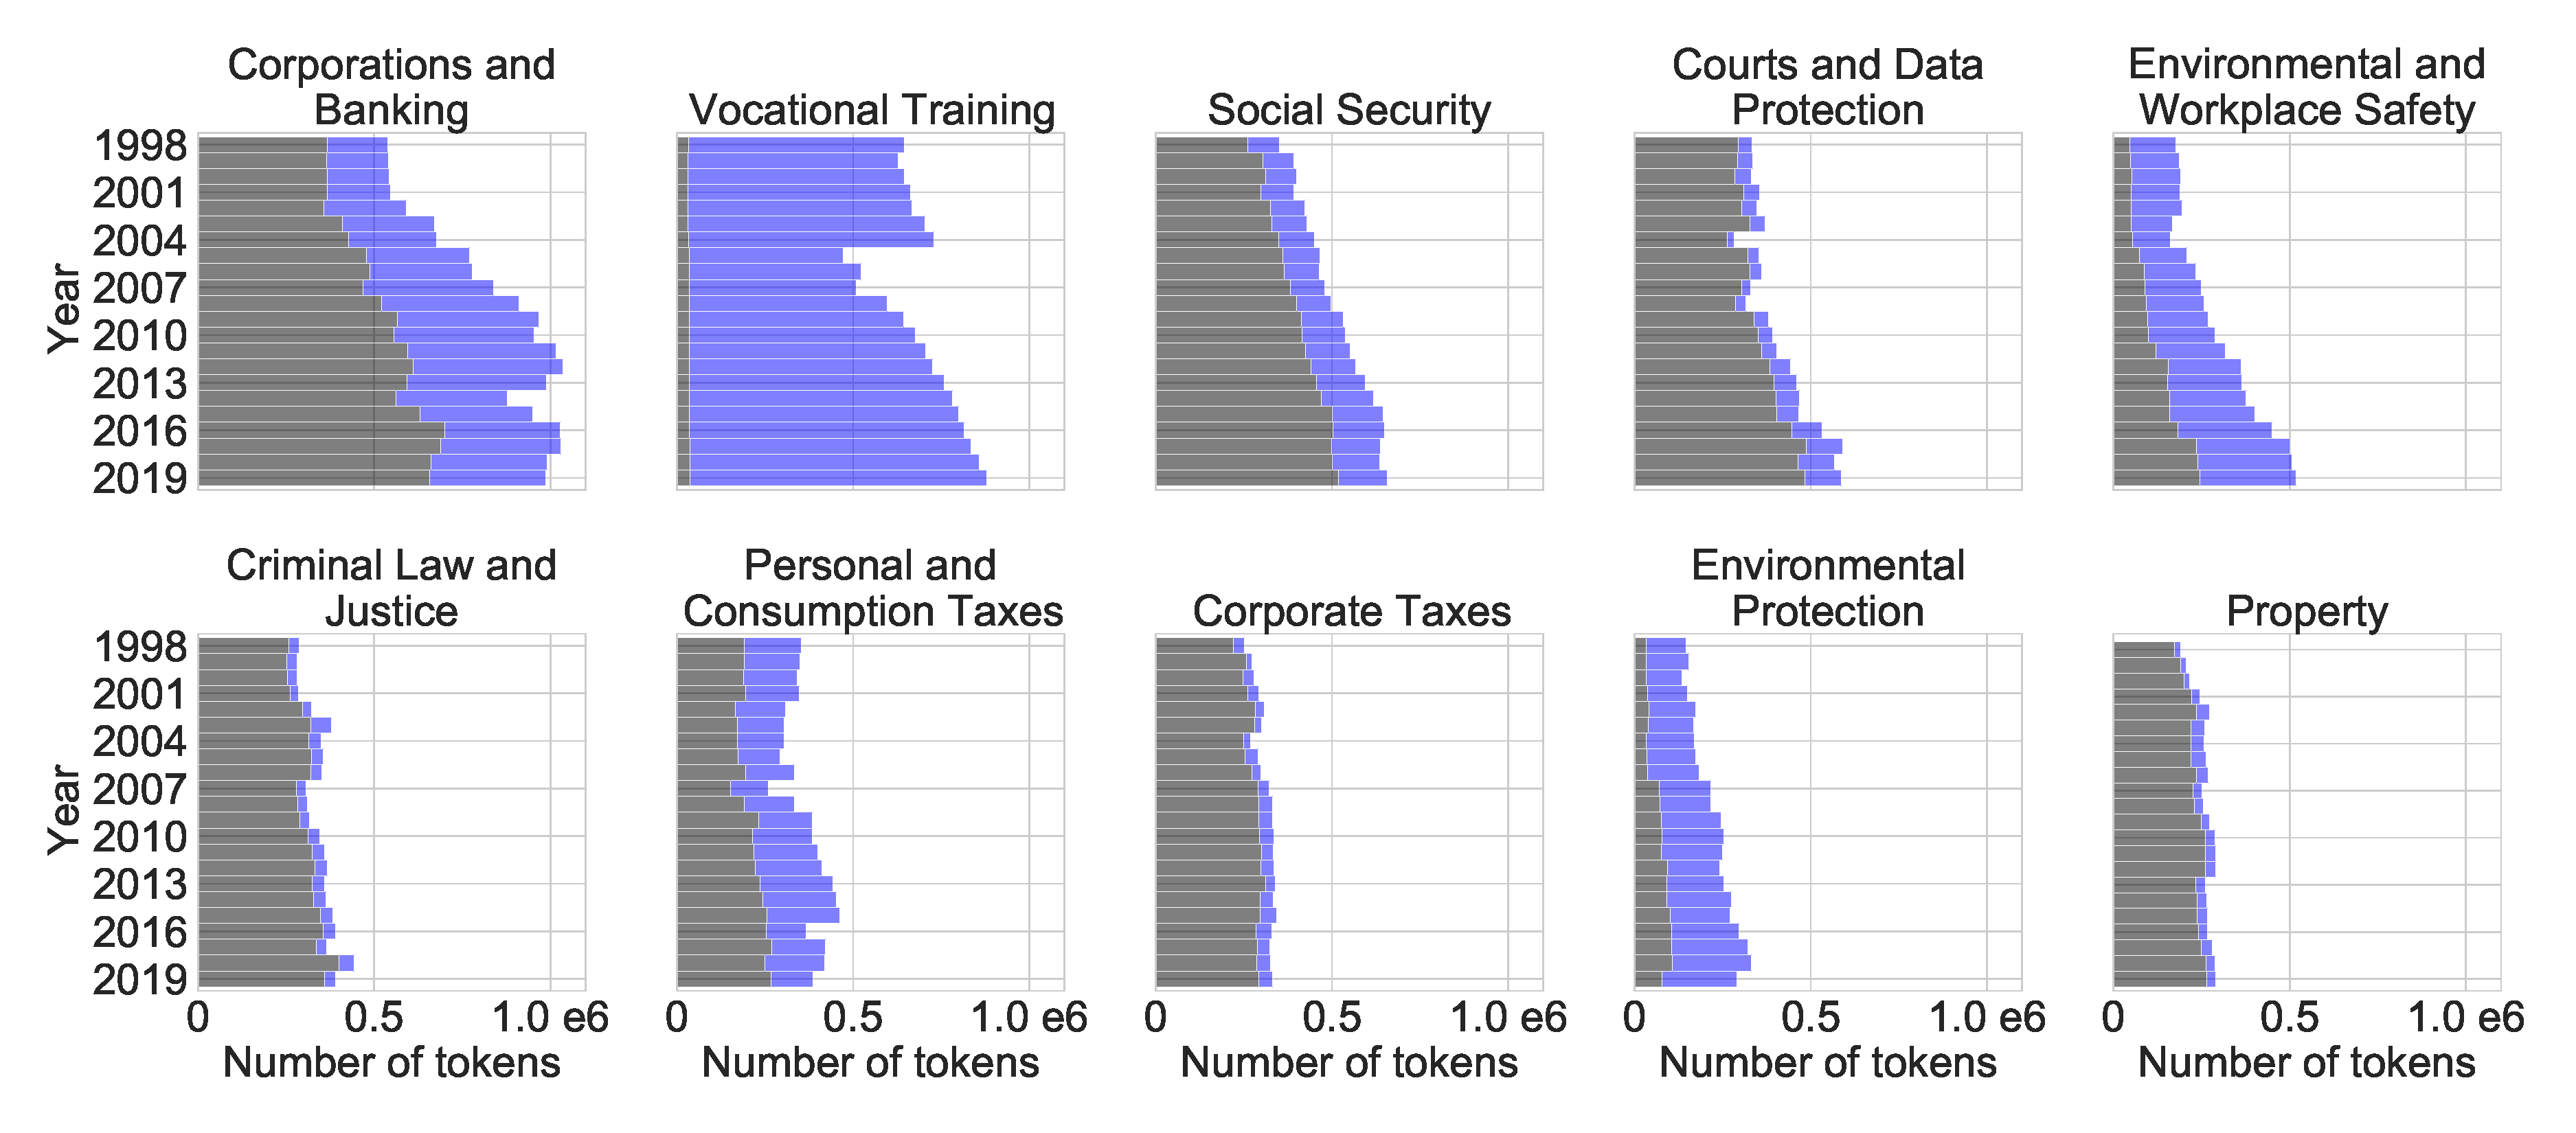
\includegraphics[width=\linewidth]{../../graphics/family-composition-absolute-n100-de.pdf}\vspace{-7pt}
	\vspace*{-6pt}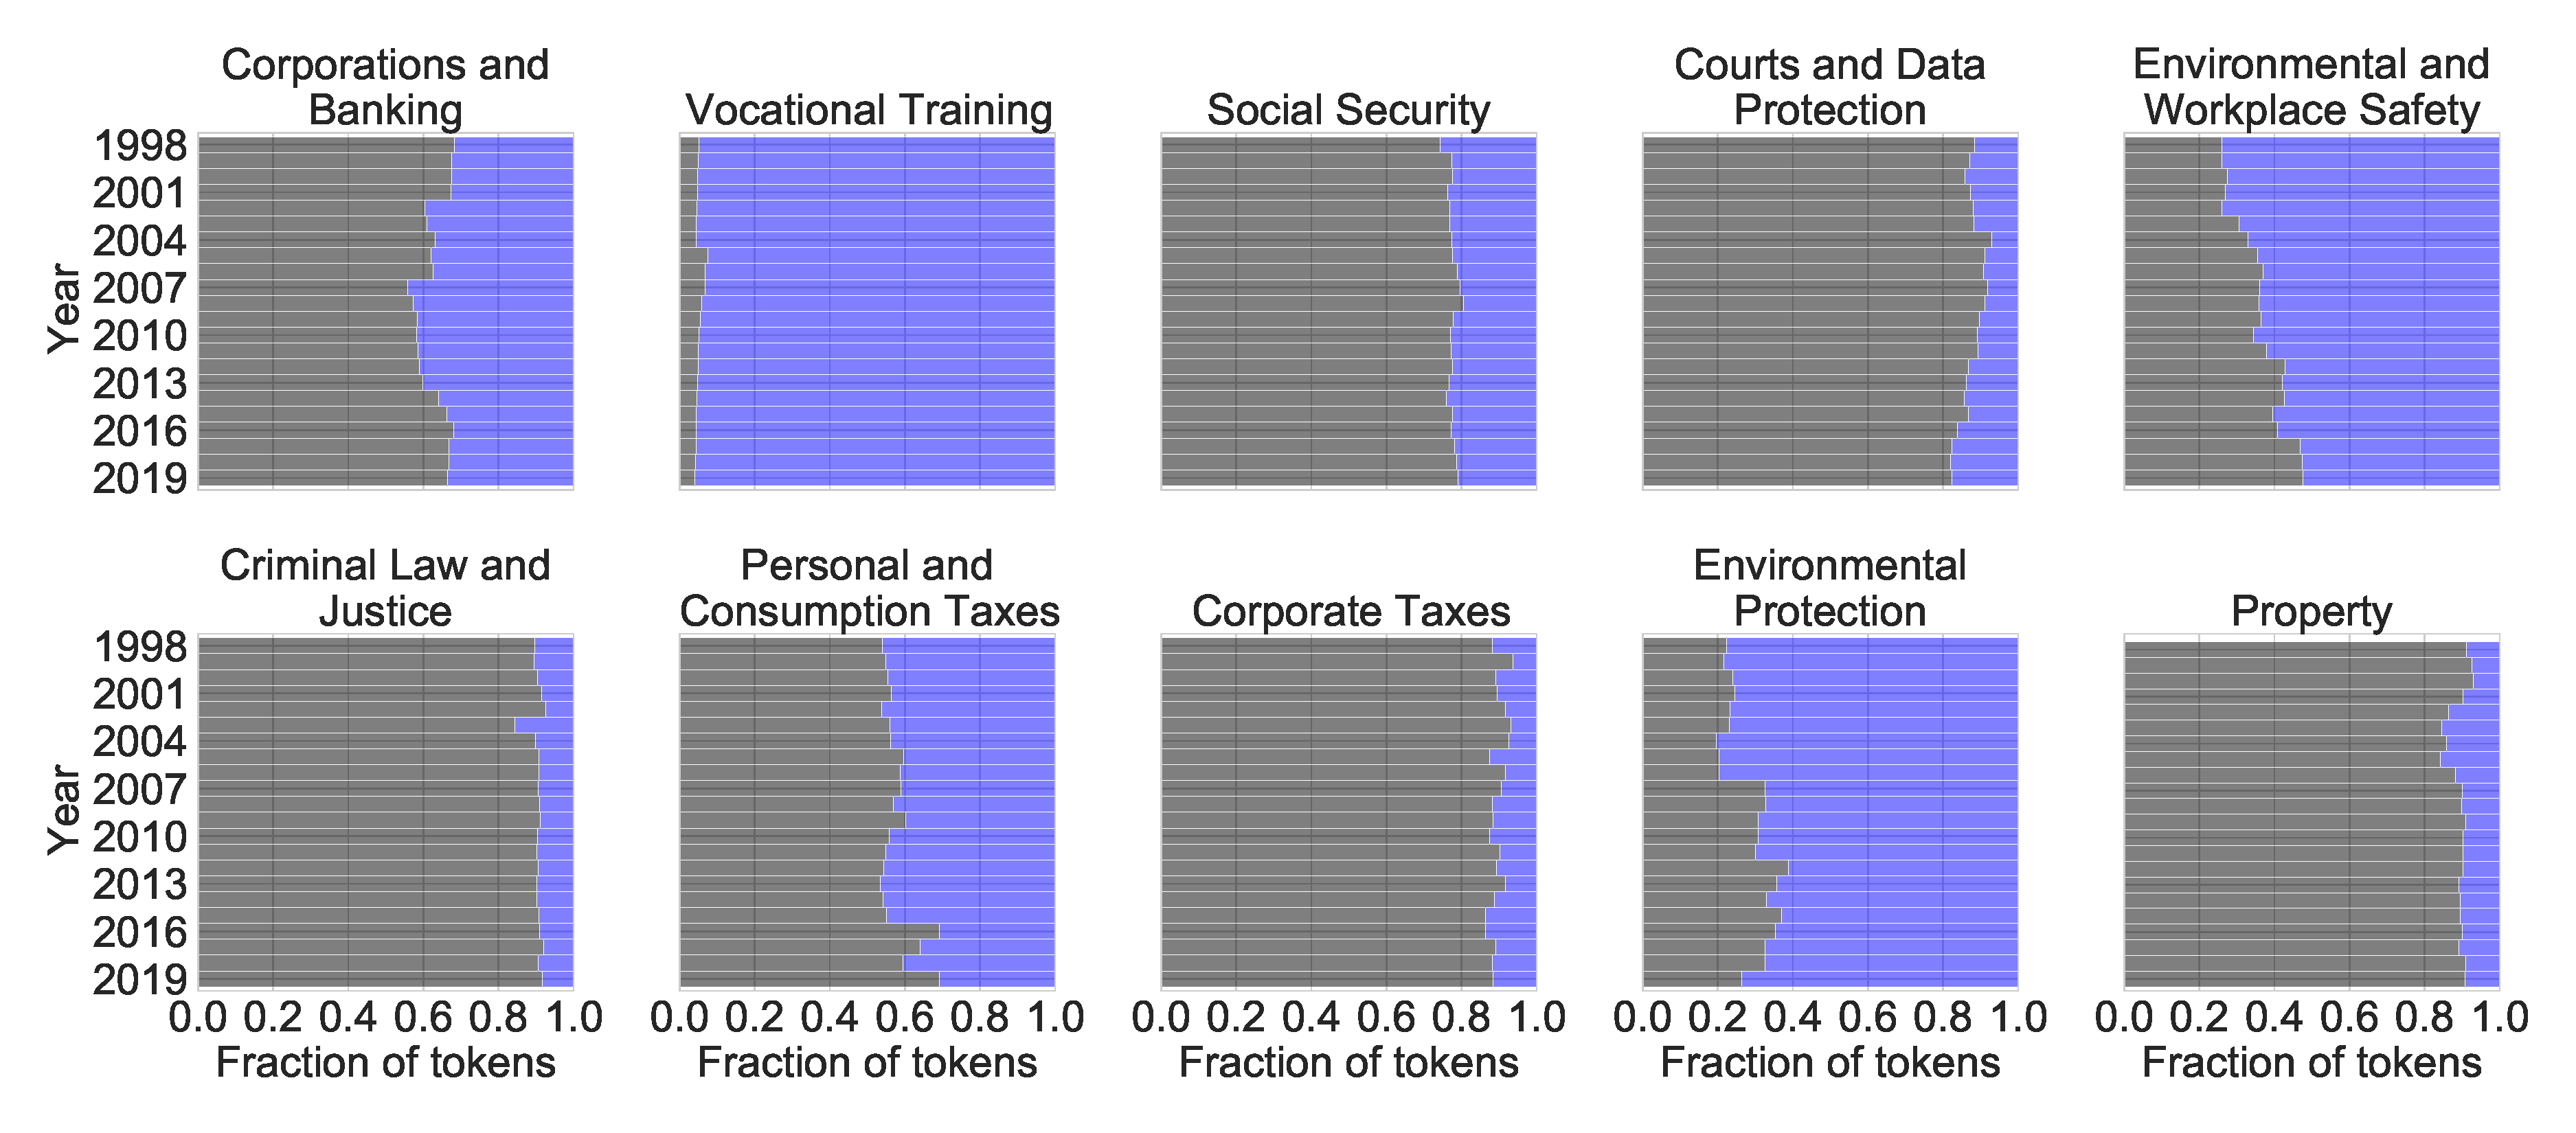
\includegraphics[width=\linewidth]{../../graphics/family-composition-relative-n100-de.pdf}%
	\subcaption{Germany}
\end{subfigure}
	\end{figure}
	
\end{document}